\section{Contenuto}
Dopo aver esaminato la \textit{vetrina} del sito passiamo ora all'analisi del contenuto. In particolare, si analizzerà la pagina di una ricetta/tecnica di cucina, in quanto è la tipologia di pagina più significativa, più numerosa e sicuramente più visitata (forse dopo la home), dato che l'obiettivo principale del sito è offrire ricette; oltre ad essa, verrà analizzata brevemente la pagina 404 ed infine anche la tipologia di pagina il cui scopo è elencare le ricette, ma nella sezione \ref{sez:ricerca}. Per esse l'analisi sarà leggermente diversa rispetto a quella effettuata per la home, in quanto l'importanza degli assi informativi cambia.

\subsection{Pagina di una ricetta}
\subsubsection{Descrizione generale}
\label{subsez:ricetta-descr}
Prenderò come esempio la pagina relativa alla (video)ricetta della parmigiana di melanzane, al link \url{https://ricette.giallozafferano.it/Parmigiana-di-melanzane.html}.
La pagina si presenta molto lunga, 22 scroll e mezzo verticali su uno schermo con risoluzione 1920x1080, con il browser in modalità non massimizzata: è un numero troppo elevato, considerando che circa solo il 42\% degli utenti fa uso di scroll nelle pagine interne; tuttavia è da considerare anche il livello di interesse dell'utente, il quale probabilmente è arrivato nella pagina perché veramente interessato ad imparare la ricetta e dunque abbastanza propenso a scrollare, pur di ricevere le informazioni che desidera.
\\~Ogni area di testo è accompagnata da un titolo descrittivo, cosa che aiuta molto il lettore: esso è però scritto in corsivo, cosa che aiuta sì il contrasto, ma diminuisce la leggibilità. 
\\~Come si può vedere in figura \ref{fig:ricetta-1}, al momento dell'ingresso nella pagina le informazioni sono quasi nulle: c'è il titolo della ricetta, il voto che gli utenti le hanno dato ed il video (solo nel caso delle video ricette, negli altri casi è presente un'immagine del piatto della stessa dimensione). Più sotto poi si intravedono le parole \textit{Difficoltà:}, \textit{Preparazione}, \textit{Cottura}, \textit{Dosi per}, \textit{Costo}: il fatto che siano tagliate può incoraggiare l'utente a fare scroll per vedere cosa c'è effettivamente sotto, il che è una buona cosa (se non le vedesse affatto sarebbe ignaro del fatto che la pagina continua). 
~\\C'è poi una cosa che rischia di creare fastidio nell'utente: nel momento in cui la pagina viene caricata, la video ricetta parte in automatico; nonostante l'audio sia di default disattivato, la cosa può stressare l'utente perché non richiesta esplicitamente. Inoltre, non appena si fa uno scroll che supera la posizione del video, esso viene spostato in basso a destra, senza venire messo in pausa: se l'utente vuole leggere la ricetta mentre guarda il video per avere delle informazioni più dettagliate può trarne beneficio, ma lasciarlo sotto gli occhi di un utente che non vi è interessato contribuisce solamente ad aumentarne lo stress e la voglia di andarsene.
~\\Come ultima cosa, vediamo che anche dopo aver fatto dello scroll, la barra superiore in cui sono contenuti logo, ricerca e collegamenti ai social, rimane staticamente attaccata alla parte alta dello schermo, comprendo informazioni potenzialmente utili.

\begin{figure}[h!]
	\centerline{
	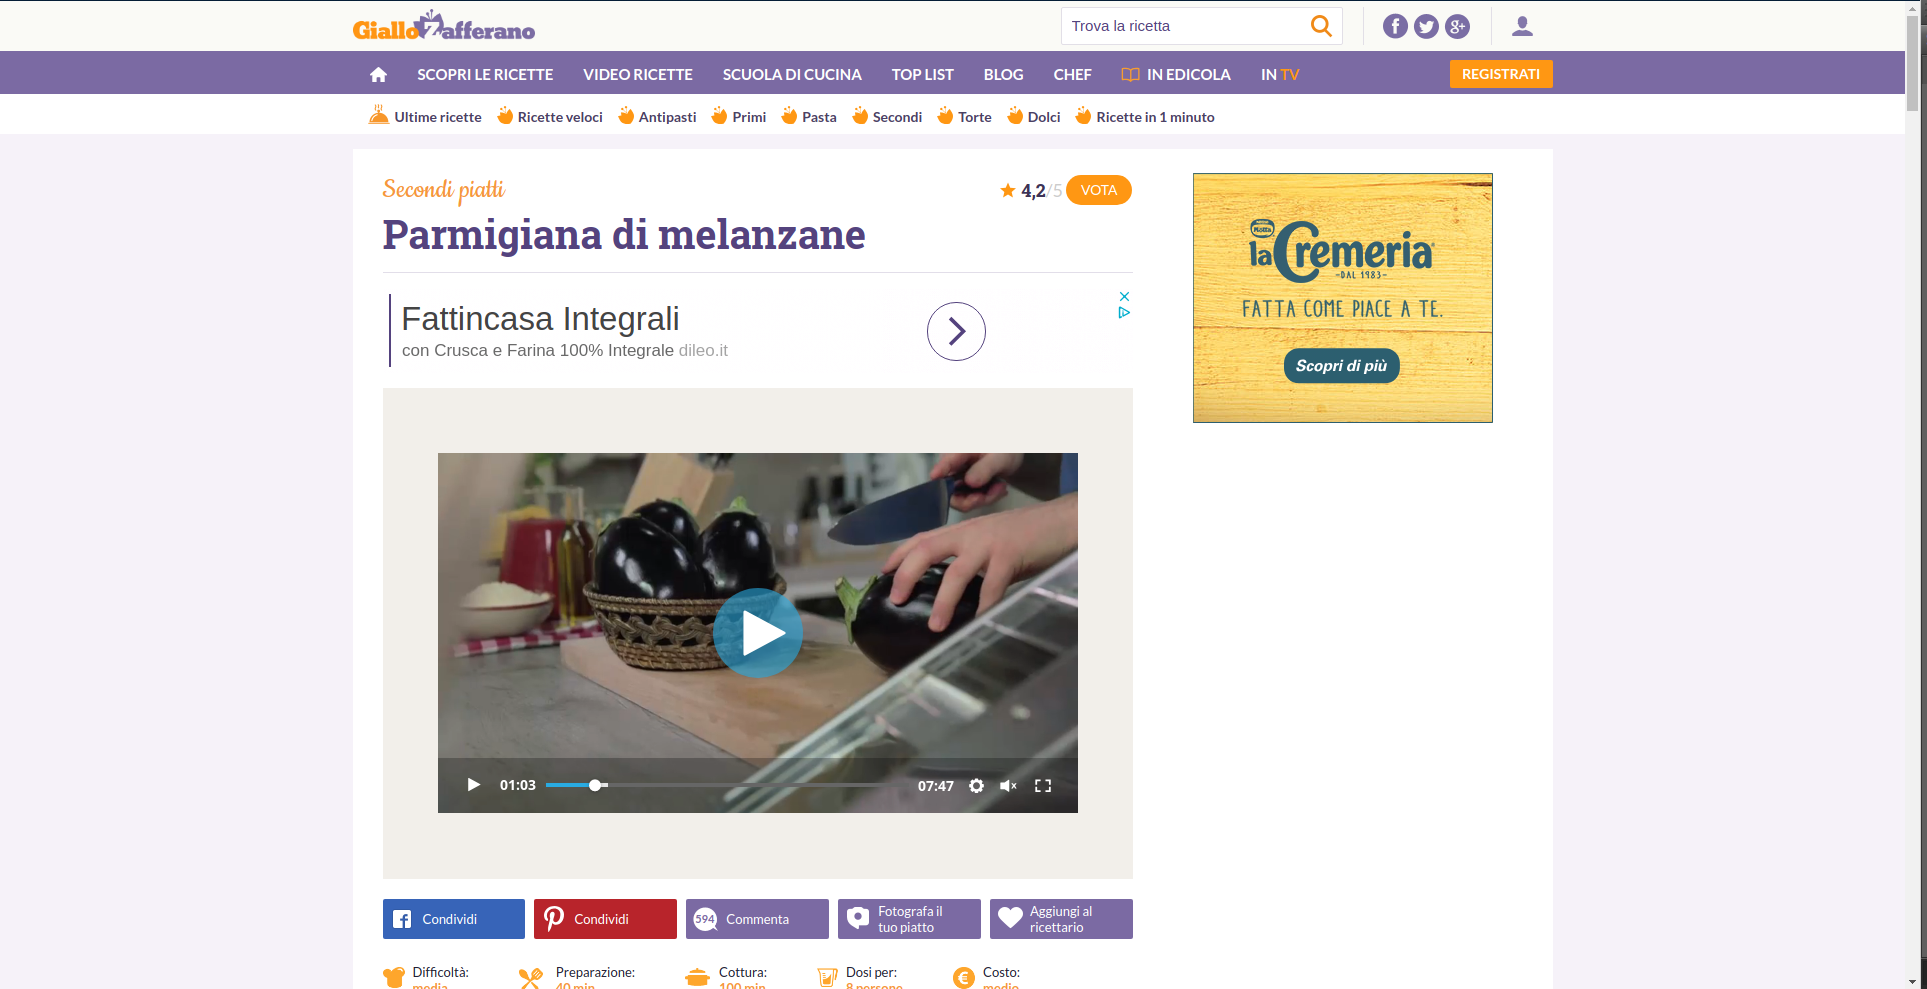
\includegraphics[scale=0.2]{images/ricetta-1.png}}
	\caption{Prima schermata della pagina ricetta della parmigiana di melanzane (ricetta-1.png) - \newline https://ricette.giallozafferano.it/Parmigiana-di-melanzane.html}
	\label{fig:ricetta-1}
\end{figure}

\newpage

\subsubsection{Le 6 W}

\paragraph{Where} 
Tale asse continua ad avere molta importanza nelle pagine interne poiché risolve il problema del \textit{lost in navigation}, permettendo di rendere chiaro all'utente il contesto in cui si trova. Dato che nel web non c'è il senso del movimento nè della bussola, utilizzare un collegamento alla home dà un orientamento "verso casa"; ciò viene fatto all'interno della pagina attraverso il logo/nome in alto a sinistra, tuttavia non è sufficiente, poiché se un utente è arrivato nella pagina attraverso il \textit{deep linking}, dargli come riferimento solo il link alla home costituisce un click sprecato e lo costringe a spostarsi dal luogo in cui c'è l'informazione di suo interesse. 
L'uso di bradcrumb avrebbe comunicato efficacemente gran parte dell'asse where, ma l'unico accenno di esso sono le parole \textit{Secondi piatti}, poste sopra al titolo della ricetta: esse sono un link che rimanda alla pagina delle ricette della categoria secondi piatti, il che può aiutare l'utente a capire parte del percorso che porta alla pagina in analisi, ma è ancora una volta un click sprecato che costringe l'utente a spostarsi.
In sostanza dunque nonostante i percorsi di navigazione siano nella home ben segnalati, rimangono difficili da ricordare una volta arrivati all'informazione ricercata.
\begin{comment}
Per non affaticare ulteriormente il visitatore ed aiutarlo a tenere a mente i percorsi fatti sarebbe stato poi opportuno colorare diversamente i link già visitati, dato che è una convenzione non standard riconosciuta in tutto il web.
\end{comment}

\paragraph{Who} 
 Anche quest'asse rimane obbligatorio nelle pagine interne, ma è sufficiente esporre il logo del sito/azienda, cosa che giallozafferano fa mantenendolo in alto a sinistra.
 
\paragraph{Why} 
L'asse why diventa nelle pagine interne opzionale ma consigliato. Come per la homepage, anche nella pagina di una ricetta esso non trova risposta, nonostante basterebbe una breve descrizione o uno slogan.

\paragraph{What} 
Tale asse rimane obbligatorio e valgono per la pagina le considerazioni fatte per la home: la presenza di riferimenti al cibo e alle ricette in tutta la pagina fanno capire che il tema è la cucina ed il titolo della ricetta aiuta a capire di essere nella pagina specifica di un piatto, anche se un utente potrebbe pensare che sia solo una pagina che descrive l'alimento e non effettivamente le procedure per la sua preparazione.

\paragraph{When}
L'asse when è opzionale e viene comunicato nello stesso modo in cui era comunicato nella home, cioè attraverso il link \textit{Ultime ricette} nel secondo menù di navigazione. 

\paragraph{How} 
Quest'asse è opzionale ma consigliato e viene solitamente soddisfatto fornendo una funzionalità di search, cosa che il sito offre posizionandola correttamente in alto a destra e anche in basso, alla fine della pagina, prima del footer.
\clearpage

\subsubsection{Schermate}
Dato che la pagina è molto lunga, la si analizzerà per schermate, a partire da quella successiva alla prima, che è già stata descritta in \ref{subsez:ricetta-descr} I blocchi di testo successivi si riferiranno sempre all'immagine sopra di loro. 


\begin{figure}[h!]
	\centerline{
	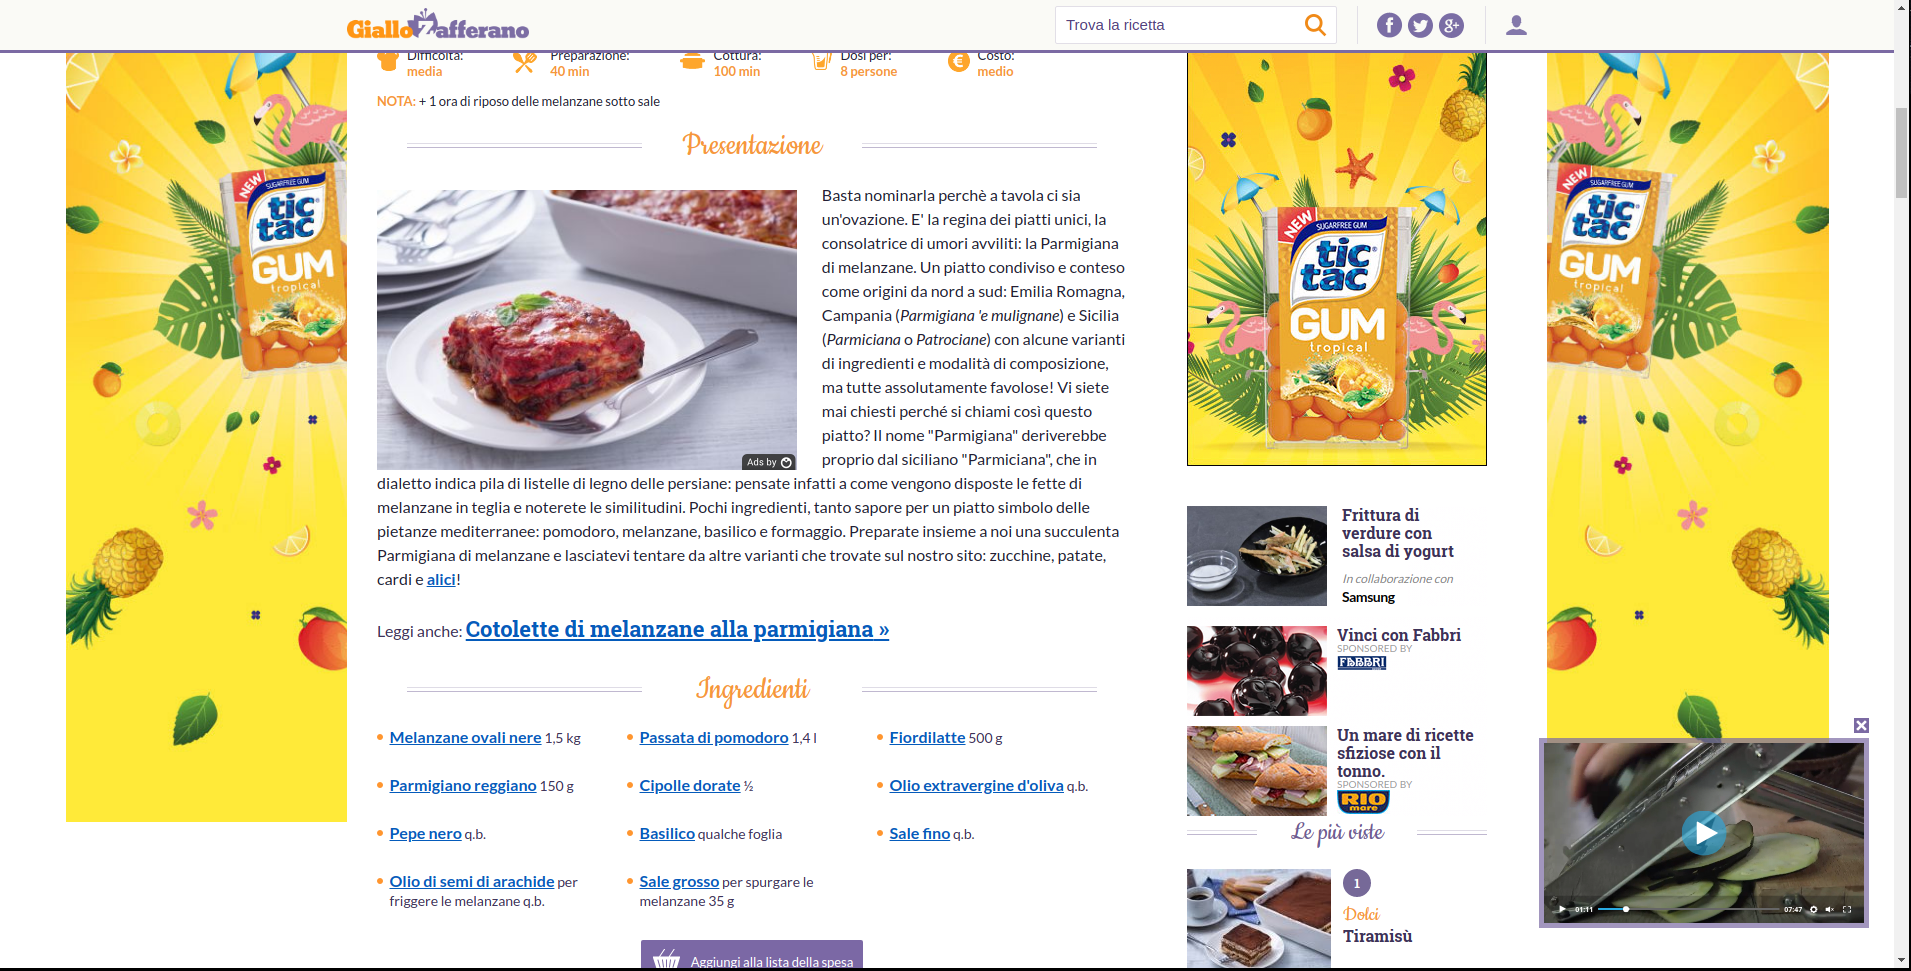
\includegraphics[scale=0.2]{images/ricetta-2.png}}
	\caption{Seconda schermata della pagina ricetta della parmigiana di melanzane (ricetta-2.png)-\newline https://ricette.giallozafferano.it/Parmigiana-di-melanzane.html}
	\label{fig:ricetta-2}
\end{figure}

In questa parte troviamo come prima cosa la \textit{Presentazione} della ricetta con solitamente una contestualizzazione storica, accompagnata da un'immagine; quest'ultima è abbastanza grande da attirare l'attenzione dell'utente, tuttavia non è cliccabile: solitamente le immagini hanno un tasso di click superiore al testo, dunque sarebbe opportuno renderla cliccabile, avendo come evento anche semplicemente l'ingrandimento della foto, per evitare che utenti inesperti perdano tempo nell'attesa di un redirect che non arriverà mai.
Per quanto riguarda il testo, anch'esso ha bisogno di miglioramenti: innanzitutto andrebbe posizionato a sinistra della foto, in modo da esaltarne l'importanza; poi andrebbe disposto in blocchi facendo uso di spazi bianchi e margini, perché com'è ora è troppo denso e viene ignorato dalla fase di scan, oltre al fatto che gli utenti apprezzano brevi frammenti d'informazione; non sono inoltre presenti alcune parole chiave, cosa che lo penalizza ancora di più nella fase di scan.
Appena sotto alla presentazione è sempre presente un riferimento ad un'altra ricetta correlata, il che può invogliare il visitatore a navigare in altre parti del sito.
Poi vediamo la sezione \textit{Ingredienti}, i quali vengono disposti su una lista divisa in 3, in cui il numero di elementi è 4, cioè il numero perfetto per non affaticare l'utente; tuttavia, dato che l'efficacia delle liste  decresce linearmente con il numero di liste disposte verticalmente, sarebbe stato meglio non dividerla, sacrificando un po' di spazio verticale in più.
\clearpage

\begin{figure}[h!]
	\centerline{
	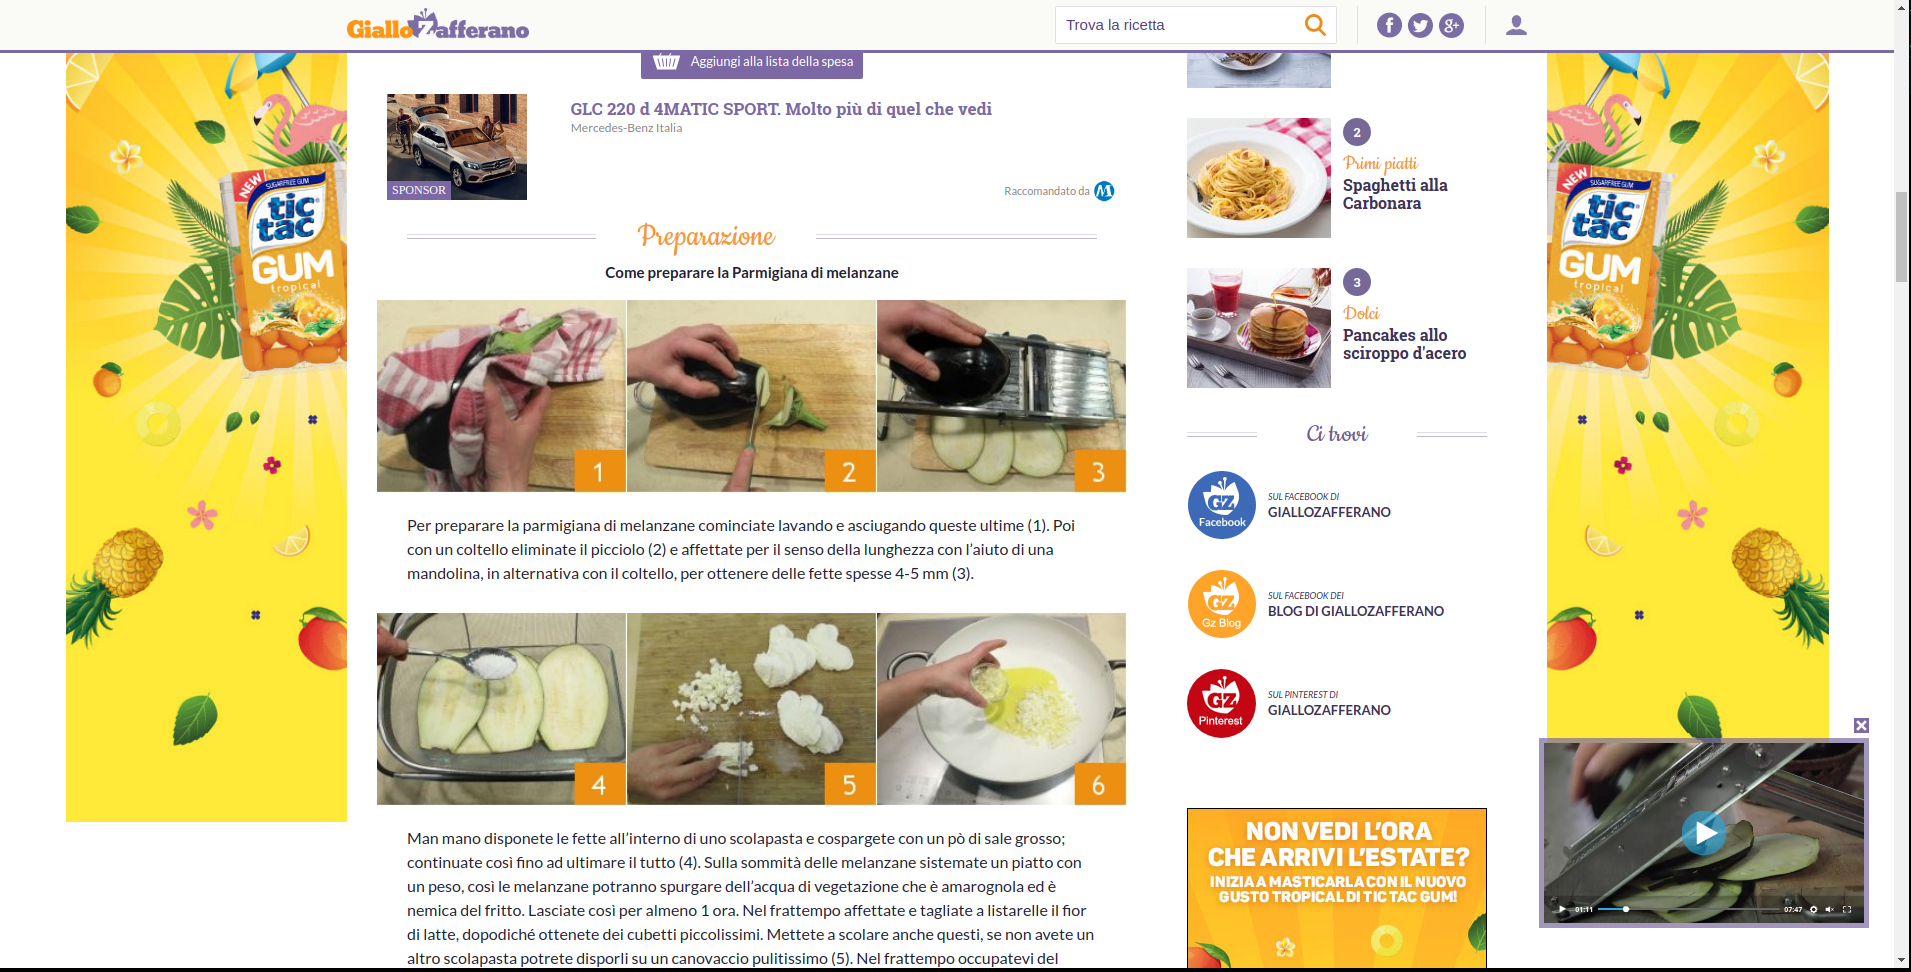
\includegraphics[scale=0.2]{images/ricetta-3.png}}
	\caption{Terza schermata della pagina ricetta della parmigiana di melanzane (ricetta-3.png)-\newline https://ricette.giallozafferano.it/Parmigiana-di-melanzane.html}
	\label{fig:ricetta-3}
\end{figure}

La successiva sezione ha come titolo \textit{Preparazione} ed è la parte più importante della ricetta; è presente un sottotitolo "Come preparare la Parmigiana di melanzane", scritto in grassetto, il quale può aiutare nella fase di scan ad identificare la sezione, qualora il titolo (che ricordo è poco leggibile perchè scritto in corsivo) non venga notato/letto. 
Ogni ricetta ha una struttura comune: il procedimento viene descritto tramite dei paragrafi di testo separati da serie di immagini, alle quali il testo fa riferimento; nonostante sia una scelta che sicuramente facilita la comprensione del procedimento, le immagini continuano a non essere cliccabili, il che comporta gli stessi problemi di cui ho parlato sotto a \ref{fig:ricetta-2}. Inoltre, è buona cosa che il testo sia diviso in blocchi, ma in esso non è presente alcuna parola chiave evidenziata, nè un titolo descrittivo: per quanto riguarda quest'ultimo, esso può non servire in questo particolare caso, dato che i blocchi sono strettamente collegati, invece le keywords mancanti sono un errore che sfavorisce lo scanning.

\clearpage

\begin{figure}[h!]
	\centerline{
	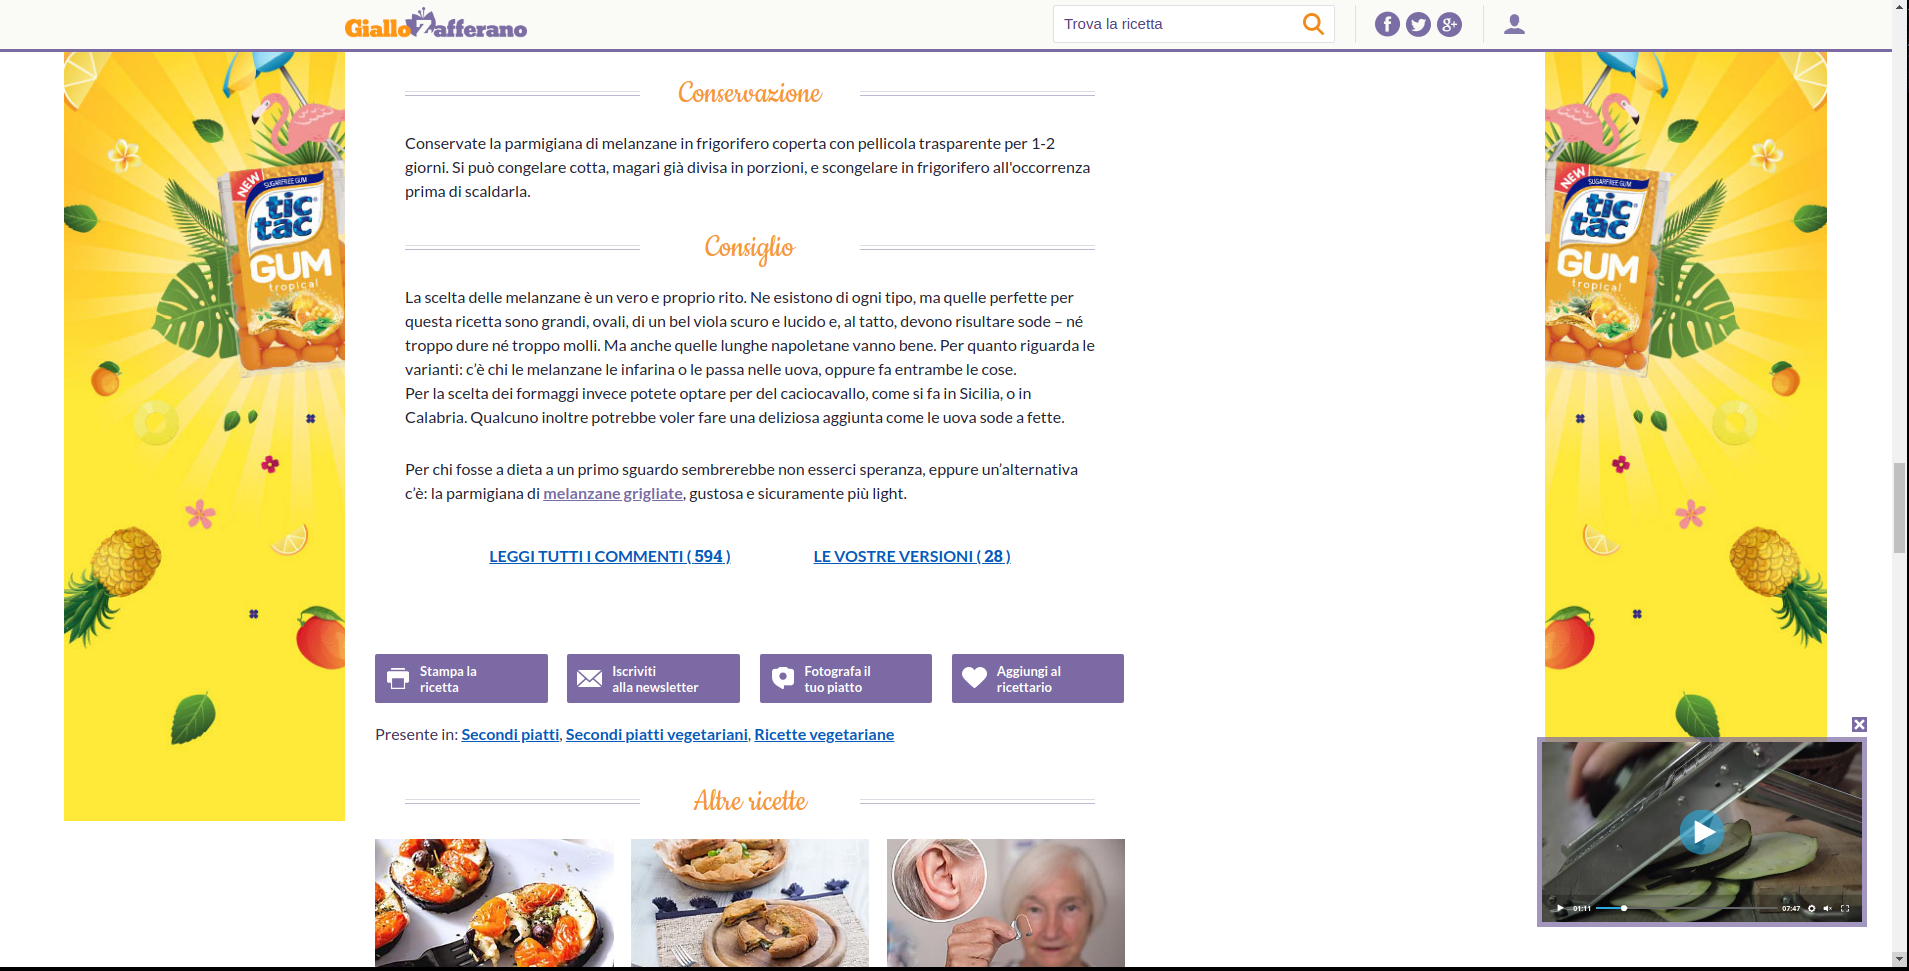
\includegraphics[scale=0.2]{images/ricetta-6.png}}
	\caption{Sesta schermata della pagina ricetta della parmigiana di melanzane (ricetta-6.png) -\newline https://ricette.giallozafferano.it/Parmigiana-di-melanzane.html}
	\label{fig:ricetta-6}
\end{figure}

Saltiamo qualche schermata dato che quarta e quinta sono identiche alla terza. Qui vediamo tre blocchi di testo abbastanza sintetici, dei quali il primo è da solo sotto il titolo \textit{Conservazione} e specifica le modalità di conservazione della pietanza, mentre gli altri due stanno sotto il titolo \textit{Consiglio}, dove vengono dati consigli relativi a questioni specifiche della ricetta. Alla luce del loro contenuto, possiamo dire che la posizione (alla fine) è  perfetta, perché sono informazioni aggiuntive di cui non tutti possono aver bisogno.
I vari blocchi facilitano lo scanning e in questo particolare caso, aver linkato \textit{melanzane grigliate}, attira sicuramente l'attenzione dell'utente.
In seguito sono presenti vari link, la maggior parte dei quali verrà probabilmente ignorata.
Notiamo poi la presenza di un accenno di breadcrumb: "\textit{presente in: secondi piatti, secondi piatti vegetariani, ricette vegetariane}" aiuta sicuramente a capire meglio la struttura e i percorsi di navigazione all'interno del sito, ma la scelta di posizionarlo così in basso è un grave errore e ne dà pochissima visibilità e quindi utilità.
\clearpage

\begin{figure}[h!]
	\centerline{
	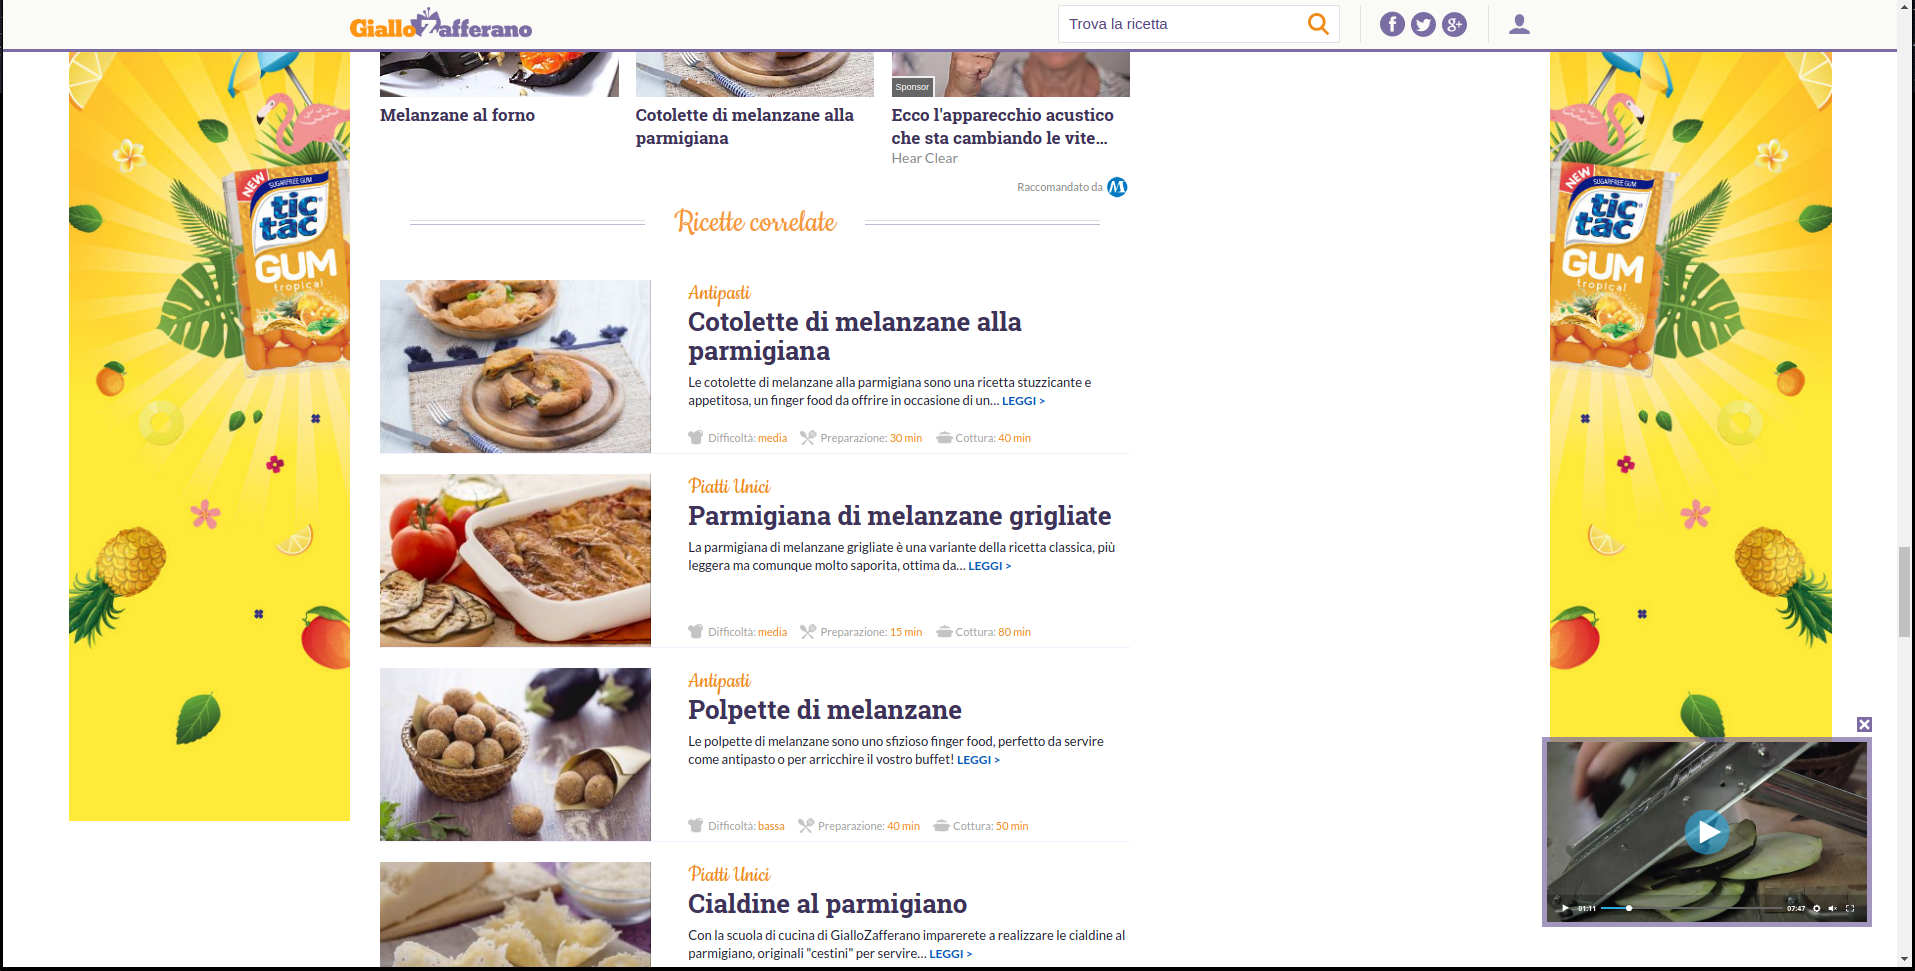
\includegraphics[scale=0.2]{images/ricetta-7.png}}
	\caption{Settima schermata della pagina ricetta della parmigiana di melanzane (ricetta-7.png) -\newline https://ricette.giallozafferano.it/Parmigiana-di-melanzane.html}
	\label{fig:ricetta-7}
\end{figure}

\begin{figure}[h!]
	\centerline{
	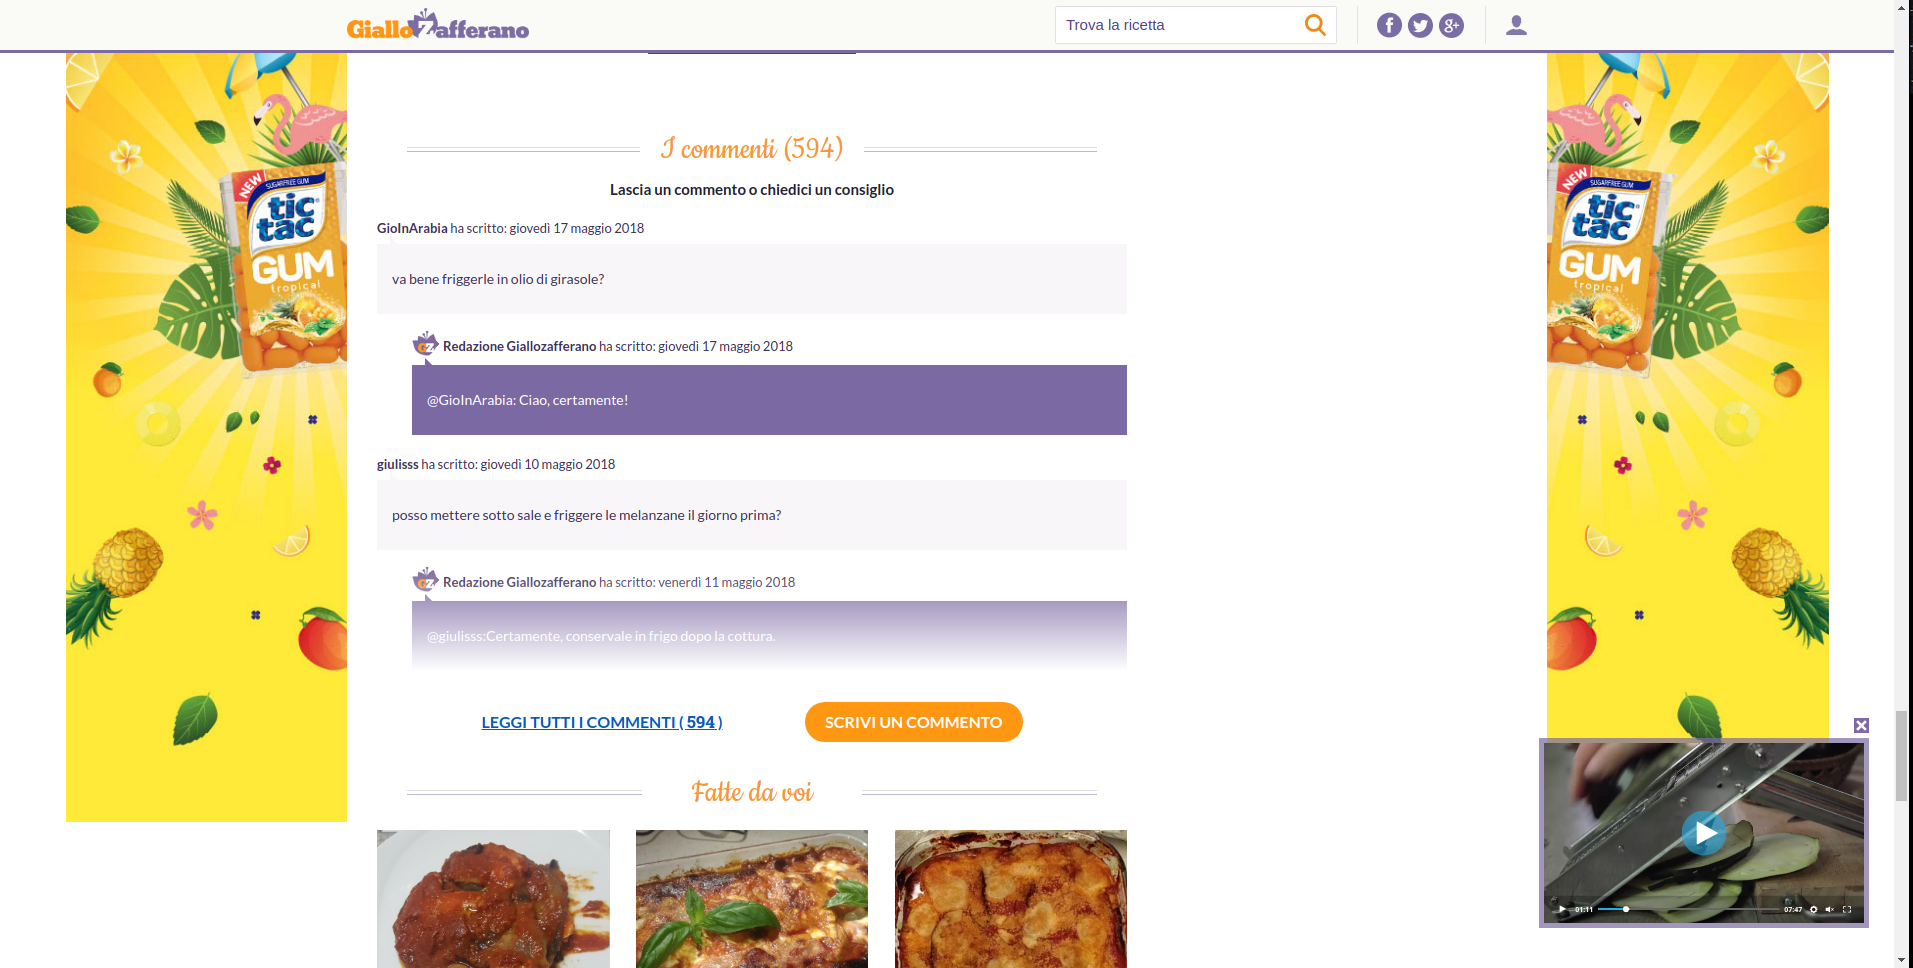
\includegraphics[scale=0.2]{images/ricetta-8.png}}
	\caption{Ottava schermata della pagina ricetta della parmigiana di melanzane (ricetta-8.png) -\newline https://ricette.giallozafferano.it/Parmigiana-di-melanzane.html}
	\label{fig:ricetta-8}
\end{figure}

In seguito vediamo la sezione "\textit{Altre ricette}" (per metà in figura \ref{fig:ricetta-6}), in cui vengono posti riferimenti ad altre ricette all'interno del sito, cosa che può invogliare l'utente a non abbandonare il sito; sono presentate come immagini disposte a griglia, cosa che permette di visualizzare più informazione in maniera compatta, anche se manda in crisi la fase di scan. 
Subito dopo appare la sezione "\textit{Ricette correlate}",che presenta ulteriori riferimenti a ricette presenti nel sito: a differenza della sezione precedente, però, l'informazione viene presentata con un layout a lista, il che può confondere l'utente, in quanto incoerente con il layout della sezione precedente.
Appena sotto c'è la sezione commenti, che finalmente riesce a dare al sito un senso di dinamicità ed aggiornamento, oltre a coinvolgere attivamente gli utenti.
Per finire, sono presenti molti altre sezioni di riferimenti a parti del sito, ma non mi ci soffermerò in quanto finirei per ripetermi. Una cosa a cui porre attenzione è invece la presenza di una barra di ricerca alla fine di tutti il contenuto: ad essa è riservata un'intera riga, tuttavia la posizione la svantaggia fortemente, dato che sicuramente sarà vista da un numero esiguo di utenti poiché, come detto in precedenza,la pagina si compone di moltissimi scroll.

\subsection{404}

\begin{figure}[h!]
	\centerline{
	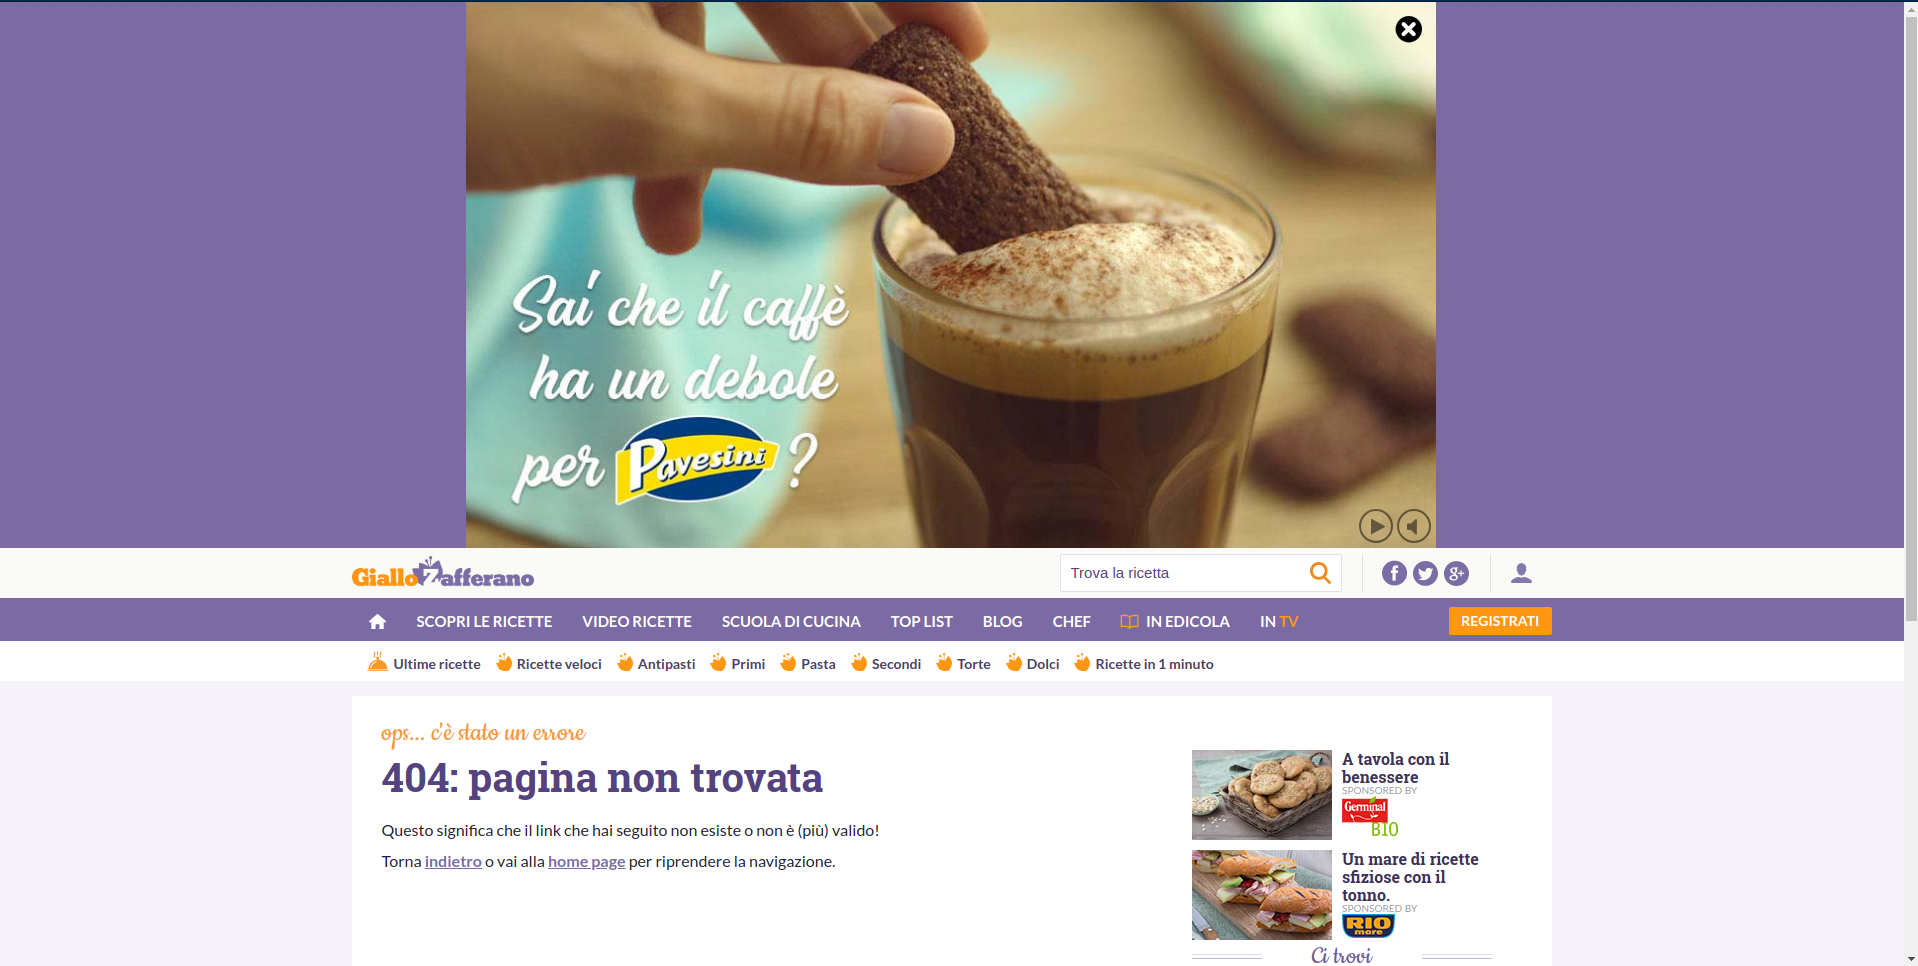
\includegraphics[scale=0.2]{images/404.png}}
	\caption{Pagina non trovata (404.png) - https://ricette.giallozafferano.it/asdasd}
	\label{fig:404}
\end{figure}

Quando l'utente medio finisce in una pagina inesistente, egli necessita di spiegazioni semplici, senza uso di tecnicismi; giallozafferano si comporta abbastanza bene, innanzitutto vediamo la scritta "\textit{ops...c'è stato un errore}", seguita dal titolo "\textit{404: pagina non trovata}". L'utilizzo del codice 404 è sconsigliato, in quanto è puramente tecnico e, nonostante molti utenti siano a conoscenza del loro significato, mediamente c'è il rischio che provochi confusione nel visitatore. Il paragrafo che segue dà però una spiegazione sintetica e comprensibile dell'errore, fornendo all'utente dei link alla home page o a alla pagina precedente: quest'ultima cosa è tuttavia rischiosa, poiché se il visitatore era arrivato alla pagina tramite il deep linking, farlo tornare indietro significherebbe farlo uscire dal sito e inoltre, nel caso in cui il visitatore avesse \textit{javascript} disattivato, tale link non avrebbe alcuna conseguenza e accrescerebbe la frustrazione dell'utente che sia aspetta un reindirizzamento.